\chapter{Electrical}
% Good reference https://www.cougarrobotics.com/wp-content/uploads/2016/11/Using-Sensors-2018.pptx.pdf

\section{Power Electronics}

\subsection{Batteries}
% Internal resistance, chemistries, ratings
Power sources are a critical component of electrical systems. For mobile ones, a battery is the obvious choice- the question is, what battery? Batteries may be rated by many parameters.

\begin{asparaenum}
  \item \textit{Chemistry} refers to the type of chemicals and technologies being used in the battery. Spillable Lead-Acid, Sealed AGM, LiPo, NiCd are all different types of chemistries on the market each with their pros and cons. Some work better at cold temperatures, some cannot be used in extremely high temperatures, and some have much higher flammability hazards. Some require maintenance and watering, some do not.
  \item \textit{Nominal voltage} is the approximate voltage that a battery will sit at. This will fluctuate throughout operation both due to internal resistance and chemical changes- over time the battery will drain and the voltage may sink. A 12 volt nominal AGM battery may be fully charged at 13.5 volts, but be depleted at 11.
  \item \textit{Amp-hours} is a measure of how much energy can be stored by the battery, specifically, how many hours it could run for if one amp was constantly being used.
  \item \textit{Cold Cranking Amps (CCA)} is a performance characteristic often found in car batteries, which must pull extremely high amounts of current in order to start an engine. As temperature negatively impacts the current-supplying ability of lead-acid batteries, the cranking capacity is usually measured at a representative worst-case temperature. The CCA rating is found by the number of amps a battery can support for 30 seconds at 0 Farenheit before the battery voltage drops to 1.2 volts per cell (7.2 volts for a 12V battery).
  \item Other measures like \textit{Pulse Cranking Amps (PCA)}, \textit{Marine Cranking Amps (MCA)}, and \textit{Hot Cranking Amps (HCA)} also exist.
  \item \textit{Internal resistance} is a key performance characteristic that is often not rated. This is a measurement that is found by realizing the battery is not an ideal voltage source, and instead modeling it as such:
  \begin{figure}[H]
    \begin{circuitikz}[american voltages]
      \fill[lightgray] (-1.6,-0.5) -- (-1.6,4.5) -- (1.6,4.5) -- (1.6, -0.5) -- cycle;
      \draw (-1.6,-0.5) -- (-1.6,4.5) -- (1.6,4.5) -- (1.6, -0.5) -- cycle;
      \draw (0,0) to [battery, l=$V_{nom}$] (0,2)
      to [R, l_=$R_{int}$] (0,4)
      to [short] (4,4)
      to [generic, l_=load] (4,0)
      to [short] (0,0);
    \end{circuitikz}
    \caption{Battery with internal resistance driving a load.}
  \end{figure}
\begin{align}
  V_{nom} - I_{load} R_{int} = V_{load} = V_{apparent}
\end{align}
  This behavior is fairly accurate: when more current is drawn, the apparent voltage of the battery will drop as well.
\end{asparaenum}

\subsection{Regulators}

\textit{Voltage regulators} help even out fluctuations in voltage, or convert between different voltage levels.

\begin{asparaenum}
  \item \textit{Linear regulators} take excess voltage and waste it as heat. They cannot step up a voltage, only decrease it. This makes them extremely inefficient, but quite cheap. 
  \item \textit{Buck converters} are a type of switching converter that has much greater efficiency, and can reduce voltage levels.
  \item \textit{Boost converters} are a type of switching converter that has much greater efficiency, and can increase voltage levels.
  \item \textit{Buck-Boost converters} are a combination of a buck and boost converter that has high efficiency, and can transform a voltage to a level either less than or higher than the input.
\end{asparaenum}

\subsection{Breakers and Fuses}

\begin{asparaenum}
  \item \textit{Fuses} are components which only permit a certain amount of current through them. Once this current is exceeded, the fuse `blows'; destroying the path where current could flow through.
  \item \textit{Slow-blow} or \textit{time-delay} fuses require this amount of current to be passed for a sustained period of time before blowing; permitting quick surge currents to pass without interruption.
  \item \textit{Breakers} serve the same role as fuses, except that they accomplish this by disconnecting the path (called `tripping') for current to flow, like a switch, rather than destroying it. They are good for applications where repeated tripping is to be expected. Normal breakers must be manually reset.
  \item \textit{Thermal breakers} will trip if abnormally high current is seen for an extended period of time, or if extremely high current (i.e. a short) is seen momentarially. This behavior makes them useful for many applications such as protecting equipment that can handle high load, but only for so long.
  \item \textit{Auto-resetting breakers} will reset on their own after allowed to cool down. This makes them useful for protecting mission-critical circuits and enabling 'retries'.
  \item \textit{Software current limits and monitoring} can be used to avoid power disruption to a circuit while still enabling safe behavior. They may be employed alongside or in lieu of fuses and breakers to provide safety functionality.
\end{asparaenum}

\subsection{Wires}

Wires seem fairly straight forward, but have their nuances.

\begin{asparaenum}
  \item Wire may be \textit{stranded} or \textit{solid}. Solid wire is often cheaper and holds its shape well, but is very difficult to form and is not good for applications where it must be flexed. For these reasons, it is relatively rare except for building wiring. Stranded wire comes in different strand counts- more strands means more flexibility (and arguably, higher current carrying ability).
  \item Wires exist with different \textit{jacketing}. The jacketing can impact flexibility as well as insulation resistance (in high voltage applications) and temperature resistance.
  \item Color is important in wires. There are different conventions which exist for different regions, industries, and companies.
  \item Wire \textit{gague} is the amount of cross-sectional area available to carry current. In the American Wire Gague (AWG) system, a lower gague number has a higher cross-sectional area. The gague should be sufficient to carry the current per safety standards, and also to minimize voltage drop. The higher the cross-sectional area, the lower the voltage drop.
\end{asparaenum}

\begin{align}
  \Delta V = I R_{wire}
\end{align}

The voltage drop can be calculated \href{https://www.calculator.net/voltage-drop-calculator.html}{\color{red}\underline{with this tool at calculator.net}}.

\section{Sensors}

\subsection{On/Off Position Sensors}
\begin{figure}[H]
\begin{subfigure}[b]{.31\linewidth}
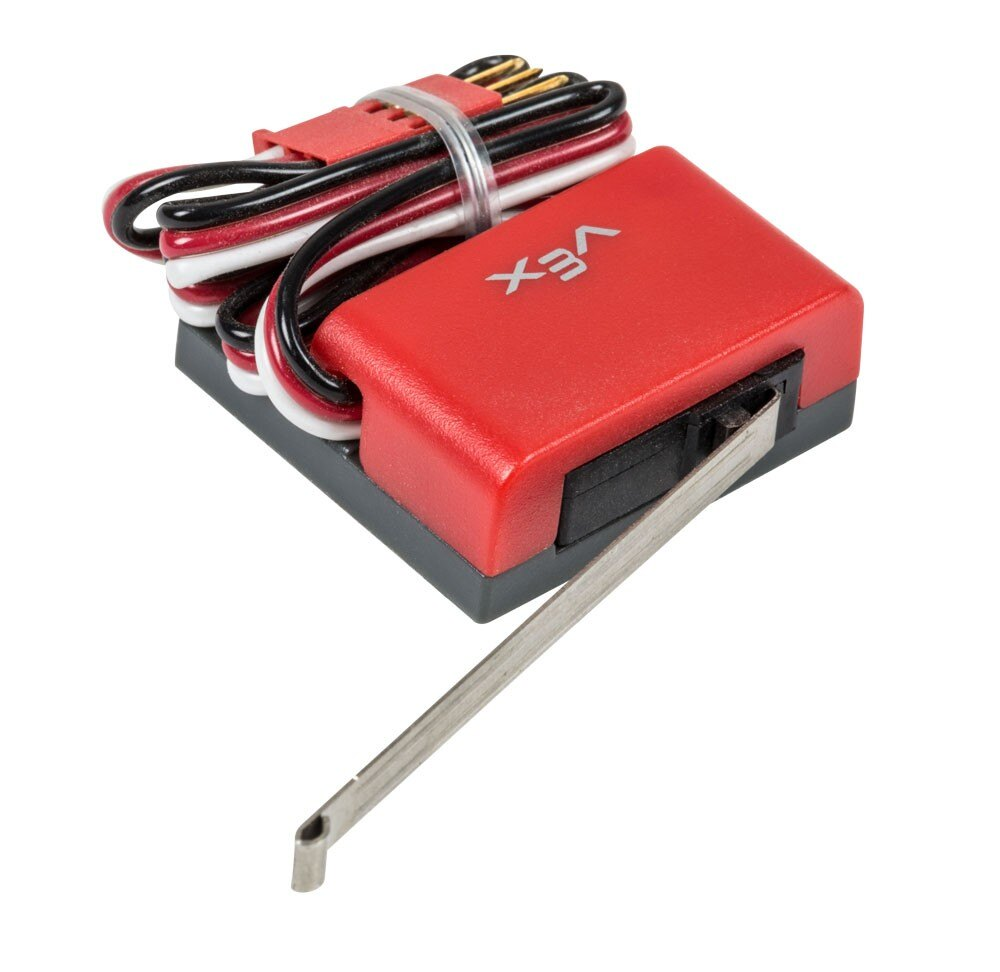
\includegraphics[width=.8\textwidth]{imgs/sensor_limitswitch.jpeg}
\subcaption{Limit Switch}
\end{subfigure}\begin{subfigure}[b]{.31\linewidth}
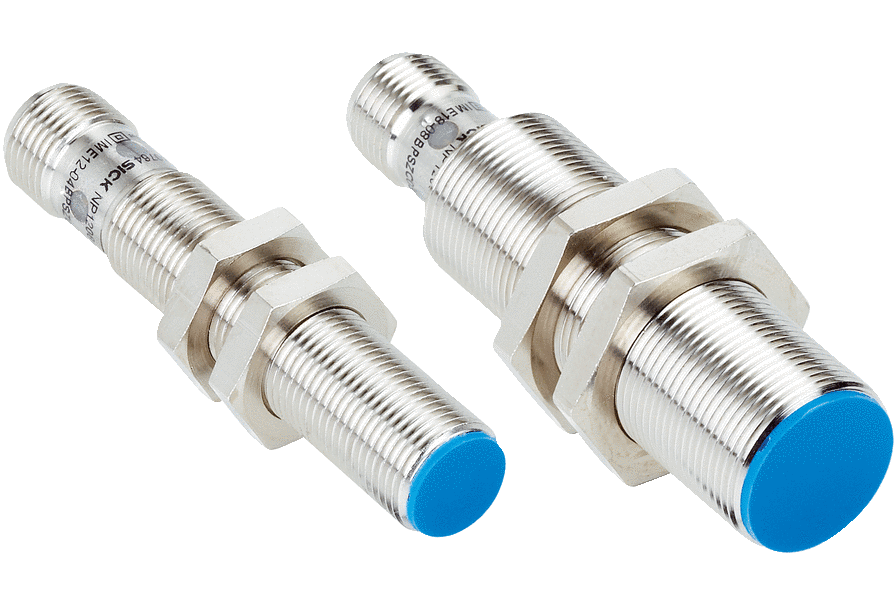
\includegraphics[width=.8\textwidth]{imgs/sensor_indprox.png}
\subcaption{Inductive Proximity Switch}
\end{subfigure}\begin{subfigure}[b]{.31\linewidth}
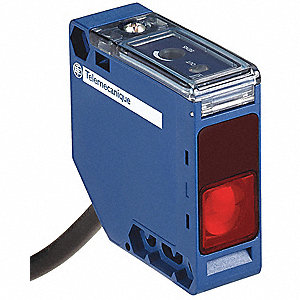
\includegraphics[width=.8\textwidth]{imgs/sensor_beambreak.jpeg}
\subcaption{IR Photoeye}
\end{subfigure}
\end{figure}

\begin{asparaenum}[a)]
\item \textit{Limit switches} are basic switches. They mechanically switch power between different positions- so do not require power to operate them (just signal).
\item \textit{Inductive proximity switches} send out a magnetic field and detect interference in this field caused by metallic objects (\textit{ferrous} metals usually work best). This allows them to sense if an object is in position without risking dangerous mechanical contact. They require appropriate power to operate (refer to their datasheet for requirements). These sensors come in different packages, although the screw-body style shown is the most common. They are also rated by their minimum and maximum sensing distances.
\item \textit{IR photoeyes} emit infrared radiation and measure how much is reflected back. This allows any object to be detected if it is within the sensing range. They require power to operate (refer to their datasheet for requirements). \item \textit{Beam breaks} emit infrared lasers and collect them on the opposite side. If an object blocks the path, the beam is broken, causing a change in signal. 
\end{asparaenum}

Switches and sensors may be denoted as [x]P[y]T to indicate how they may be wired. For example, a \textit{SPDT}, or \textit{Single-Pole Double-Throw} switch has a single contactor which can be switched between two positions. A \textit{DPST} may only alternatve the switch between a connected and unconnected state (single pole) but has a second electrically isolated version of the switch (double-throw).

Switches also may be \textit{momentary}, reverting state as soon as they are unpressed, or \textit{toggle}, staying put until actively switched back (like a lightswitch, or a pushbutton pen). If the switch is momentary, it may be either \textit{normally open (NO)} or \textit{normally closed (NC)}, referring to if the switch is open or closed by default. If the switch has two poles, the poles may be referred to as NO and NC as one will be normally opened, and one normally closed.

Sensors can be wired in various ways.

\begin{figure}[H]
\begin{subfigure}[b]{.4\linewidth}
\begin{circuitikz}[american voltages] \draw
  (0,0) node[ground]{} to [R] (0,2)
  to [push button, *-o] (0,4) node[left]{$V$};
  \draw (+2,2) node[below]{To input} to [short] (0,2);
\end{circuitikz}
\subcaption{Pull-Down Wiring}
\end{subfigure}\begin{subfigure}[b]{.4\linewidth}
\begin{circuitikz}[american voltages] \draw
  (0,0) node[ground]{} to [push button] (0,2)
  to [R, *-o] (0,4) node[left]{$V$};
  \draw (+2,2) node[below]{To input} to [short] (0,2);
\end{circuitikz}
\subcaption{Pull-Up Wiring}
\end{subfigure}

\begin{subfigure}[b]{.47\linewidth}
\begin{circuitikz}[american voltages]

    \fill[gray] (-1,1)--(-3,1)--(-3,3)--(-1,3)--cycle;
    \draw[black] (-1,1)--(-3,1)--(-3,3)--(-1,3)--cycle;

    \node[black] at (-2,2){PNP Sensor} ;

  \draw (1.5,0) node[ground]{} to [R, -*] (1.5,2);1
  \draw (-1,2) -- (2,2) node[above]{To input};
  \draw (-1,1.5) -- (0,1.5) -- (0,0) node[ground]{};
  \draw (-1,2.5) -- (0,2.5) to [short, -o] (0,4) node[left]{$V$};
\end{circuitikz}
\subcaption{PNP Sensor Wiring}
\end{subfigure}\begin{subfigure}[b]{.47\linewidth}
\begin{circuitikz}[american voltages]

    \fill[gray] (-1,1)--(-3,1)--(-3,3)--(-1,3)--cycle;
    \draw[black] (-1,1)--(-3,1)--(-3,3)--(-1,3)--cycle;

    \node[black] at (-2,2){NPN Sensor} ;

  \draw (1.5,4) node[left]{$V$} to [R, o-*] (1.5,2);
  \draw (-1,2) -- (2,2) node[below]{To input};
  \draw (-1,1.5) -- (0,1.5) -- (0,0) node[ground]{};
  \draw (-1,2.5) -- (0,2.5) to [short, -o] (0,4) node[left]{$V$};
\end{circuitikz}
\subcaption{NPN Sensor Wiring}
\end{subfigure}
\caption{Sensor wiring diagrams.}
\end{figure}

\begin{asparaenum}[a)]
\item \textit{Pull down resistors} make the inputs of a microprocessor rest naturally at ground level. When the connected switch is closed, the resistance of the switch is much much less than the pulldown resistor, so the voltage of the input will rise to the logic voltage. The resistor is sized so as not to consume too much current (usually R = 5 to 20 k$\Omega$). A microprocessor may have such a resistor built-in to the circuitry, although the resistor may need to be enabled.
\item \textit{Pull up resistors} work on the same principle as pull down resistors but with reversed voltages. On the RoboRIO, 2.2 k$\Omega$ pull-up resistors are on all DIO pins when in input mode.
\item \textit{NPN} and \textit{PNP} sensors are to be wired as shown. You may note that the wiring looks the same as for a pull-up or pull-down, respectively; match the type of pulling resistor in your microprocessor to the type of sensor you intend to use, otherwise external pulling resistors may be necessary.
\end{asparaenum}



% Wiring schemes (pull up vs pull down)

\subsection{Variable Position Sensors}
\begin{figure}[H]
\begin{subfigure}[b]{.45\linewidth}

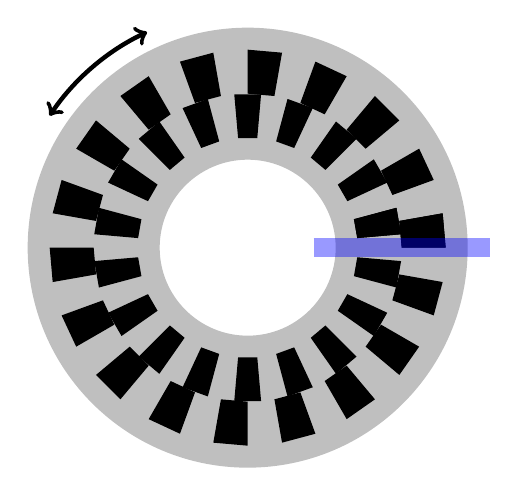
\begin{tikzpicture}[x=1.1in, y=1.1in]
  \fill[lightgray, even odd rule] (0,0) circle[radius=1] circle[radius=0.4];
  \foreach \x in {0,...,18} 
    \fill[black] ({0.9*cos(\x*20)}, {0.9*sin(\x*20)}) -- ({0.7*cos(\x*20)}, {0.7*sin(\x*20)}) -- ({0.7*cos(\x*20+10)}, {0.7*sin(\x*20+10)}) -- ({0.9*cos(\x*20+10)}, {0.9*sin(\x*20+10)}) -- cycle ;
  \foreach \x in {0,...,18} 
    \fill[black] ({0.5*cos(\x*20+5)},  {0.5*sin(\x*20+5)})  -- ({0.7*cos(\x*20+5)},  {0.7*sin(\x*20+5)}) 
              -- ({0.7*cos(\x*20+15)}, {0.7*sin(\x*20+15)}) -- ({0.5*cos(\x*20+15)}, {0.5*sin(\x*20+15)}) -- cycle ;
  \draw[blue, line width=7, opacity=0.4] (0.3,0) -- (1.1,0);
  \draw[black, <->, ultra thick] (-0.9,0.6) arc (146.3:115:1.081);
  
  
\end{tikzpicture}

\subcaption{Encoder}
\end{subfigure}\begin{subfigure}[b]{.45\linewidth}

\begin{tikzpicture}[x=1.1in, y=1.1in]
  \fill[white, opacity=0] (0,0) circle[radius=1];
  \fill[olive] ({cos(200)}, {sin(200)}) arc (200:-20:1) -- 
               ({0.7*cos(-20)}, {0.7*sin(-20)}) arc(-20:200:0.7) -- cycle;

  \draw ({0.85*cos(-20)}, {0.85*sin(-20)}) to [short, *-o] ({0.85*cos(-20)}, {0.85*sin(-20) - 0.25}) node[below]{$V$};
  \draw ({0.85*cos(200)}, {0.85*sin(200)}) to [short, *-] ({0.85*cos(200)}, {0.85*sin(200) - 0.25}) node[ground]{};
  \draw[line width=7] (0,0)--({0.85*cos(130)}, {0.85*sin(130)});
  \draw[black, <->, ultra thick] (-0.9,0.6) arc (146.3:115:1.081);
  \draw (0,0) to [short, *-o] (0, -0.25) node[below]{signal};
\end{tikzpicture}

\subcaption{Potentiometer}
\end{subfigure}
\caption{Position sensors.}
\end{figure}

\begin{asparaenum}[a)]
\item \textit{Encoders} use rotating discs with multiple on/off positions in them to determine position. The on/off mechanism could be optical, magnetic, or something else entirely. A microprocessor running fast enough can watch the waveform produced by the encoder and determine how much the position has changed. Some encoders have builtin microprocessors, which can feed back more complex signals, while others may simply feed back \textit{quadrature} data from the two channels that are monitored. This data takes the form of a square wave.

\begin{figure}[H]
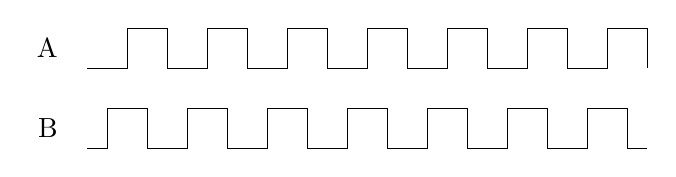
\begin{tikzpicture}[x=0.4in, y=0.4in]

\node[black, left] at (0, 0.25){B};
\draw (0.25,0)
\foreach \x in {0,...,6} {
  -- (\x+0.5, 0) -- (\x+0.5, 0.5) -- (\x+1, 0.5) -- (\x+1, 0)
} -- (7.25,0);

\node[black, left] at (0, 1.25){A};
\draw (0.25, 1)
\foreach \x in {0,...,6} {
  -- (\x+0.75, 1) -- (\x+0.75, 1.5) -- (\x+1.25, 1.5) -- (\x+1.25, 1)
} ;
\end{tikzpicture}
\caption{Encoder waveform}
\end{figure}

If the encoder spins one direction, the waveform for A will lead that of B. If it goes the other direction, B will lead A. Unless specified as an \textit{absolute} encoder, encoders are \textit{relative} devices, meaning that they can only keep track of changes, so will not maintain state when power is cycled. \textit{Homing}, the process of moving a mechanism until a hard stop or limit switch is hit, is required to establish a known position upon startup.

If only speed data is need (i.e. for the tachometer of a car, where the engine never reverses direction), a single channel can be used.

\item \textit{Potentiometers} have a resistive element, with the moving wiper making contact somewhere in the middle of it. When the wiper moves, the resistance between the wiper and the ends changes, which allows the voltage to be read. These are inherently absolute sensors- power cycling does not affect the resistance values. \textit{Multi-turn} potentiometers allow the shaft to be rotated multiple times by running the wiper through a helical spiral. Linear potentiometers also exist- they often come in a piston-style package that can be mounted with rod ends.
\end{asparaenum}

\subsection{Vision}

\begin{figure}[H]
\begin{subfigure}[b]{.19\linewidth}
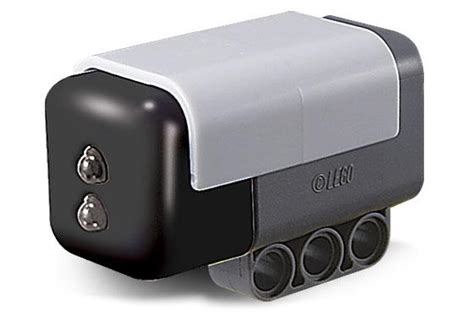
\includegraphics[height=0.9in]{imgs/sensor_color.jpeg}
\subcaption{Light/Color Sensor}
\end{subfigure}\begin{subfigure}[b]{.19\linewidth}
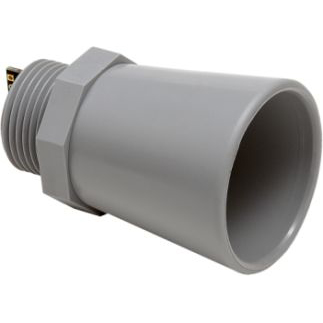
\includegraphics[height=0.9in]{imgs/sensor_ultrasonic.jpeg}
\subcaption{Ultrasonic Sensor}
\end{subfigure}\begin{subfigure}[b]{.19\linewidth}
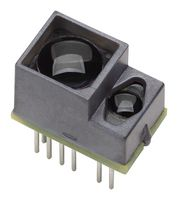
\includegraphics[height=0.9in]{imgs/sensor_tof.jpeg}
\subcaption{Time of Flight Sensor}
\end{subfigure}\begin{subfigure}[b]{.19\linewidth}
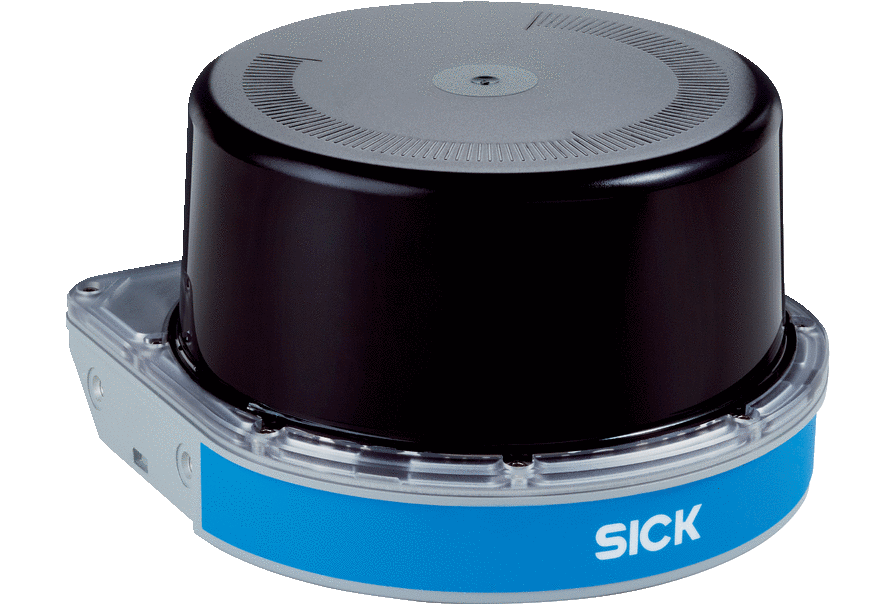
\includegraphics[height=0.9in]{imgs/sensor_lidar.png}
\subcaption{LIDAR}
\end{subfigure}\begin{subfigure}[b]{.19\linewidth}
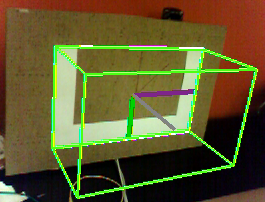
\includegraphics[height=0.8in]{imgs/sensor_cv.png}
\subcaption{Computer Vision}
\end{subfigure}
\caption{Sensors for giving a sense of vision.}
\end{figure}

\begin{asparaenum}[a)]
\item \textit{Light and color sensors} have a simple photoreciever which picks up light. This light may either be \textit{ambient} or produced by the sensor itself and reflected back. Calibration of color sensors is very important to gaining consistent readings, as unlike full-blown computer vision, shape and context are not (inherently) available.
\item \textit{Ultrasonic sensors} send out high-pitched sound waves and measure how long it takes for them to return. These can be finnicky, and do not work to detect objects that absorb, rather than reflect sound.
\item \textit{Time of flight} sensors work on the same principle as ultrasonic sensors, but with light. Light travels much, much faster- so these devices are more sophisticated and expensive.
\item \textit{LIDAR} systems employ a moving time of flight sensor to build a 3D map of the surroundings.
\item \textit{Computer Vision (CV)} can be used to pick up targets visually and determine their distance and relative position. It's particularly easy when the targets are a specialized color and shape that is distinct from everything else. CV systems can operate on even the simplest of hardware such as a smartphone, but the latency and image quality may suffer. Specialized sensors exist to improve the key performance parameters when using a camera in a real-time system.
\end{asparaenum}

\subsection{Inertial Measurement}
Measurement of position in 3D space can be established alternatively by measuring accelerations and magnetic fields.

\begin{asparaenum}[a)]
\item \textit{Gyroscopes} measure the rate of rotational acceleration. They can be used to find rotational velocity and position by performing numeric integration with a computer. As the rotational acceleration/velocity on a rigid body is constant, it does not matter where they are mounted so long as it is of sufficient rigidity and vibration isolation.
\item \textit{Accelerometers} measure linear acceleration. They can be used to find linear velocity and position by performing numeric integration with a computer.
\item \textit{Magnetometers} or \textit{digital compasses} pick up magnetic fields (such as the earth's). This allows them to determine absolute orientation, although magnetic fields can be greatly disturbed by metallic structures and buildings.
\item \textit{Integrated Motion Units} combine several of these sensors into one system, complete with an onboard microprocessor to perform aforementioned numerical integration. This dedicated processing allows them to acheive high integration accuracy.
\end{asparaenum}


\section{Terminals and Connectors}

\begin{figure}[H]
\begin{subfigure}[b]{.24\linewidth}
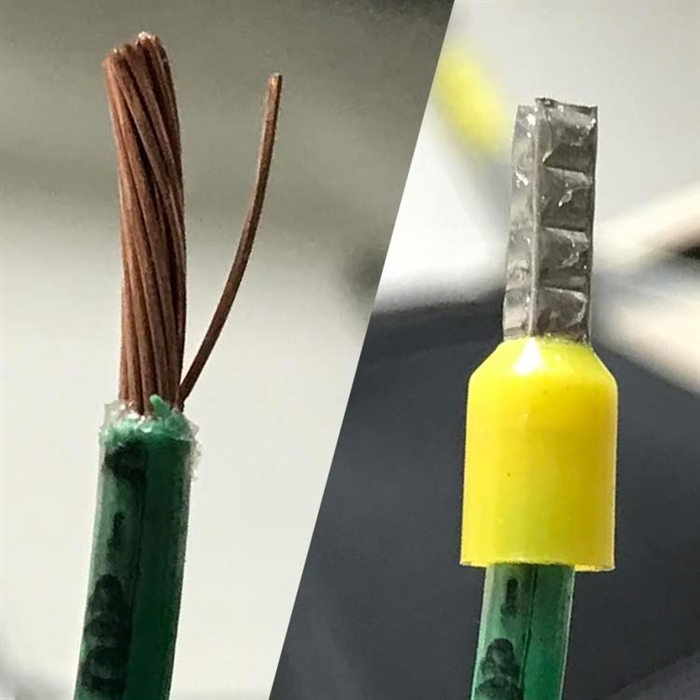
\includegraphics[height=0.9in]{imgs/connector_ferrule.jpeg}
\subcaption{Ferrule}
\end{subfigure}\begin{subfigure}[b]{.24\linewidth}
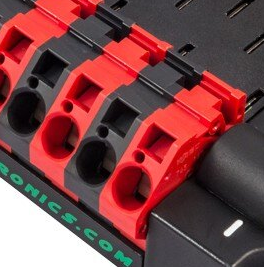
\includegraphics[height=0.9in]{imgs/connector_wago.jpeg}
\subcaption{WAGO Connector}
\end{subfigure}\begin{subfigure}[b]{.24\linewidth}
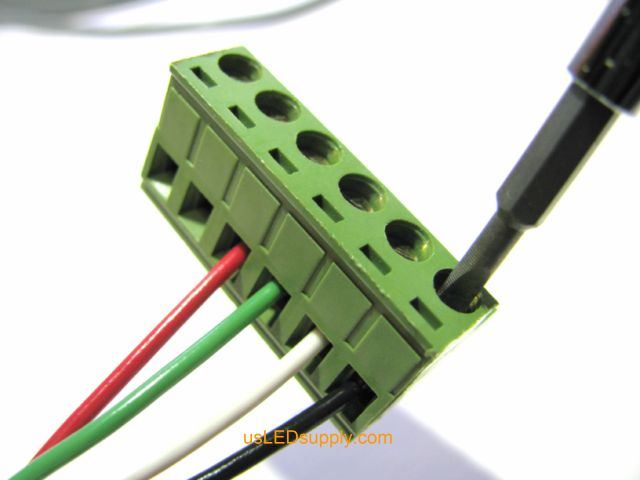
\includegraphics[height=0.9in]{imgs/connector_screwterm.jpeg}
\subcaption{Screw-Down Terminal}
\end{subfigure}
\caption{Simple wire connections.}
\end{figure}

\begin{asparaenum}[a)]
  \item \textit{Ferrules} are crimped onto the ends of stranded wire to prevent fraying.
  \item \textit{WAGO connectors} are spring loaded, with the user being able to insert a wire by use of a prying tool to open the jaws and inserting the wire before removing the tool. By their spring-loaded nature, they are very resistant to vibration. These can be somewhat annoying to use, especially in tight spaces.
  \item \textit{Screw-down terminals} are common for industrial use, although they are not as resistant to vibrations, but are quite easy to use.
\end{asparaenum} 

\begin{figure}[H]
\begin{subfigure}[b]{.24\linewidth}
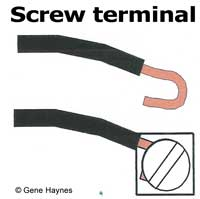
\includegraphics[height=0.9in]{imgs/connector_solidwire.jpeg}
\subcaption{Screw-down terminal with bare wire}
\end{subfigure}\begin{subfigure}[b]{.24\linewidth}
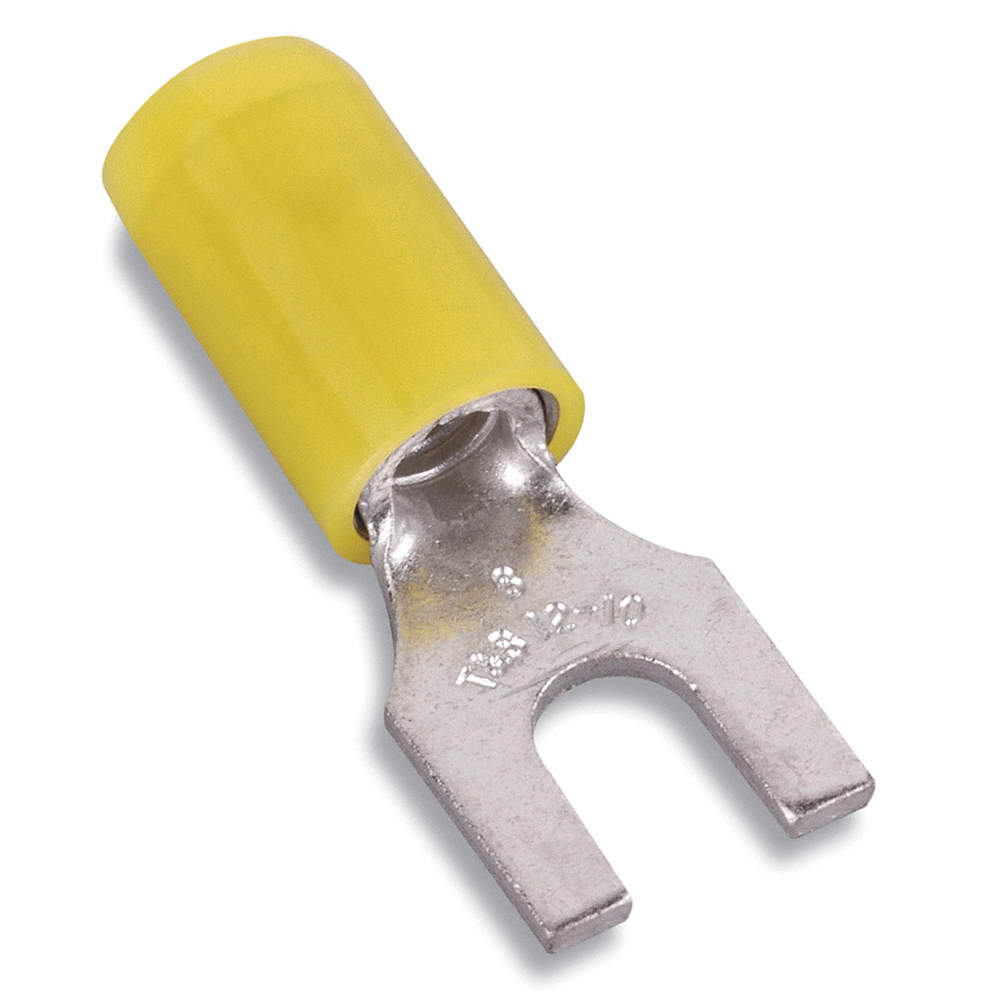
\includegraphics[height=0.9in]{imgs/connector_fork.jpeg}
\subcaption{Fork Terminal}
\end{subfigure}\begin{subfigure}[b]{.24\linewidth}
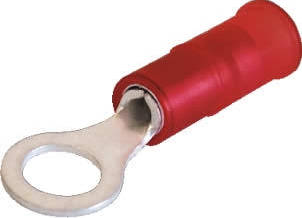
\includegraphics[height=0.9in]{imgs/connector_ring.jpeg}
\subcaption{Ring Terminal}
\end{subfigure}
\caption{Screw terminal connections.}
\end{figure}

\begin{asparaenum}[a)]
  \item \textit{Screw terminals} can accept hooked solid-core wire as shown. Make sure you hook the wire in the direction indicated to make sure the wire will tighten on installation instead of straightening.
  \item \textit{Fork terminals} crimp around a wire, and are well-suited to such screw terminals as they do not require full removal of the screw in order to be installed.
  \item \textit{Ring terminals} crimp around a wire, and work with screw terminals or even with bolt-and-hole applications. They are positive- they cannot be tugged off as a fork terminal might be.
\end{asparaenum} 

All screw based terminals, however, are subject to loosening under vibration, making them suboptimal for automotive or other mobile applications.

\begin{figure}[H]
\begin{subfigure}[b]{.24\linewidth}
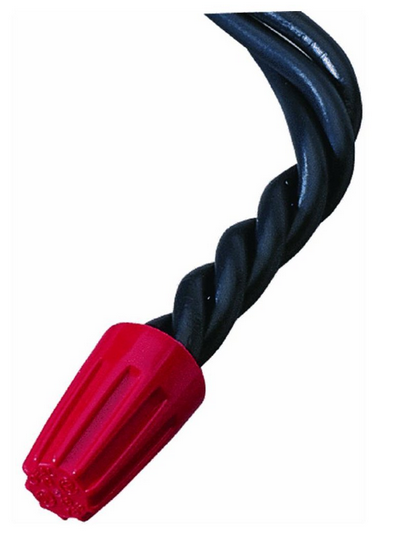
\includegraphics[height=0.9in]{imgs/connector_wirenut.jpeg}
\subcaption{Wire Nut}
\end{subfigure}\begin{subfigure}[b]{.24\linewidth}
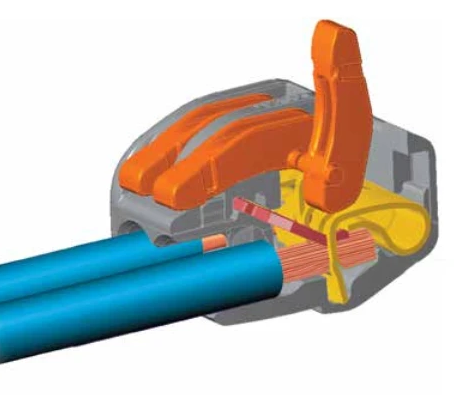
\includegraphics[height=0.9in]{imgs/connector_levernut.png}
\subcaption{Lever Nut}
\end{subfigure}\begin{subfigure}[b]{.24\linewidth}
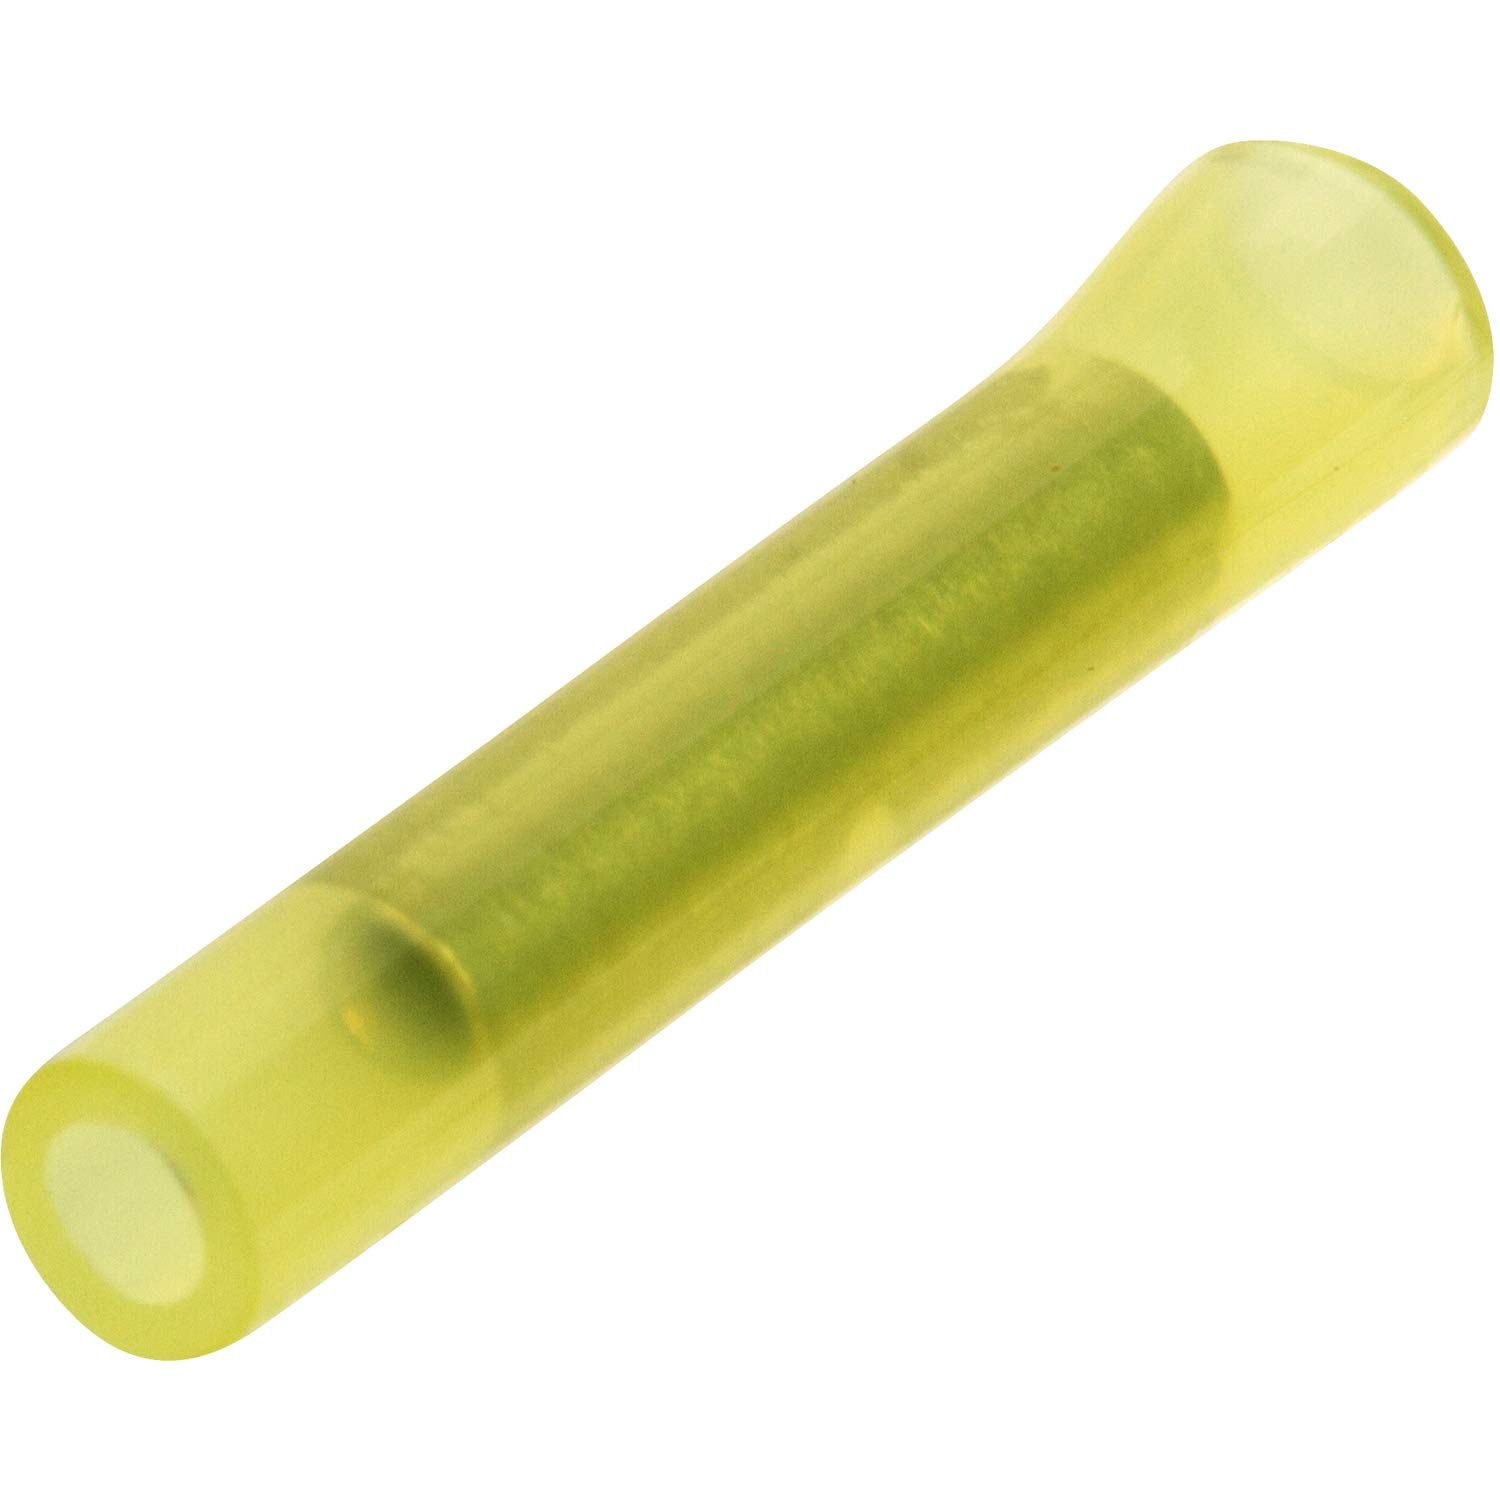
\includegraphics[height=0.9in]{imgs/connector_buttsplice.jpeg}
\subcaption{Butt Splice}
\end{subfigure}
\caption{Wire-to-wire connectors.}
\end{figure}

\begin{asparaenum}[a)]
  \item \textit{Wire nuts} go over top of twisted pairs of wires to connect them more securely than simply taping them together. Very common in building wiring, but not good for anything that would see vibrations.
  \item \textit{Lever nuts} allow wires to be separately joined together and quite easily. The installation process is as easy as opening a lever, inserting a wire, and closing the lever. Of course since they are multiple parts, they can be quite expensive.
  \item \textit{Butt splices} are crimped over two wires to join them together.
\end{asparaenum} 

\begin{figure}[H]
\begin{subfigure}[b]{.24\linewidth}
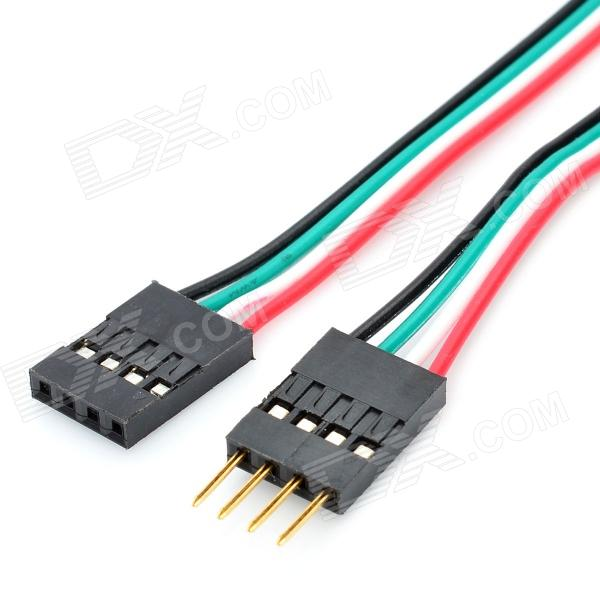
\includegraphics[height=0.9in]{imgs/connector_headers.jpeg}
\subcaption{Servo/Header Pins}
\end{subfigure}\begin{subfigure}[b]{.24\linewidth}
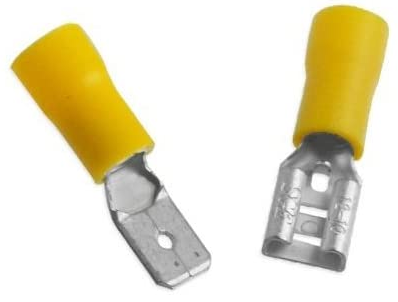
\includegraphics[height=0.9in]{imgs/connector_tabbed.png}
\subcaption{Tabbed Connector}
\end{subfigure}\begin{subfigure}[b]{.24\linewidth}
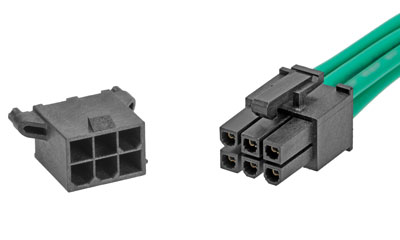
\includegraphics[height=0.9in]{imgs/connector_minifit.jpeg}
\subcaption{Locking Connector}
\end{subfigure}\begin{subfigure}[b]{.24\linewidth}
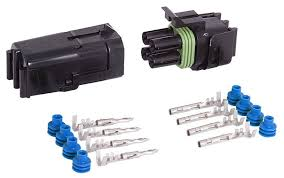
\includegraphics[height=0.9in]{imgs/connector_weatherpack.jpeg}
\subcaption{Waterproof Connector}
\end{subfigure}

\begin{subfigure}[b]{.24\linewidth}
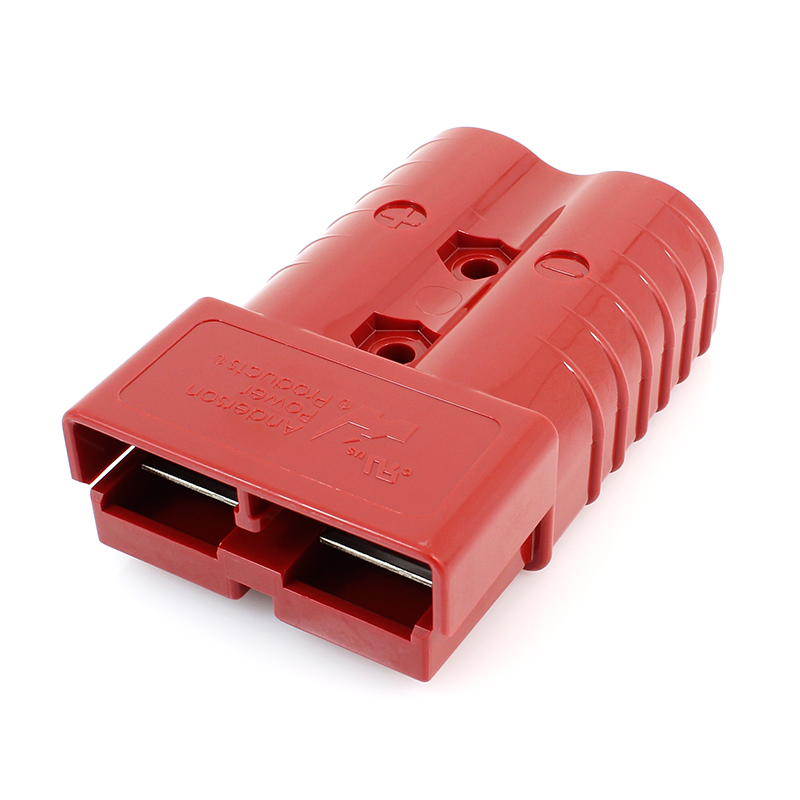
\includegraphics[height=0.9in]{imgs/connector_anderson.png}
\subcaption{Anderson Connector}
\end{subfigure}\begin{subfigure}[b]{.24\linewidth}
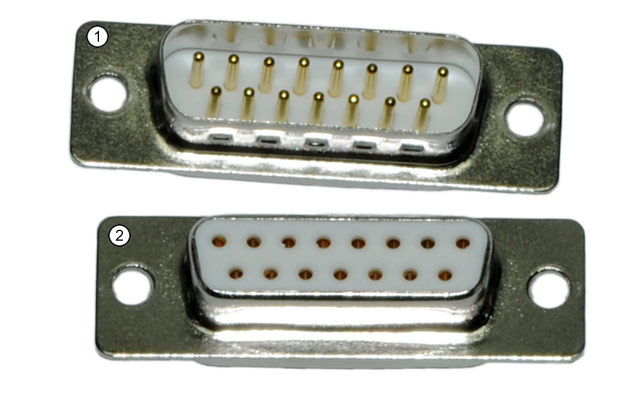
\includegraphics[height=0.9in]{imgs/connector_dsub.jpeg}
\subcaption{D-sub Connector}
\end{subfigure}\begin{subfigure}[b]{.24\linewidth}
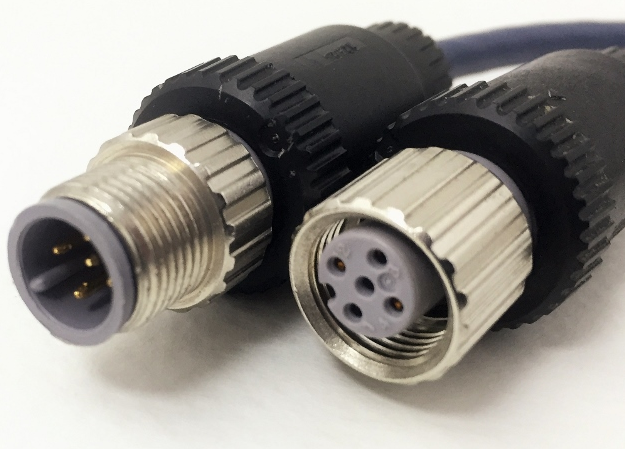
\includegraphics[height=0.9in]{imgs/connector_screw.png}
\subcaption{Screw on Connector}
\end{subfigure}\begin{subfigure}[b]{.24\linewidth}
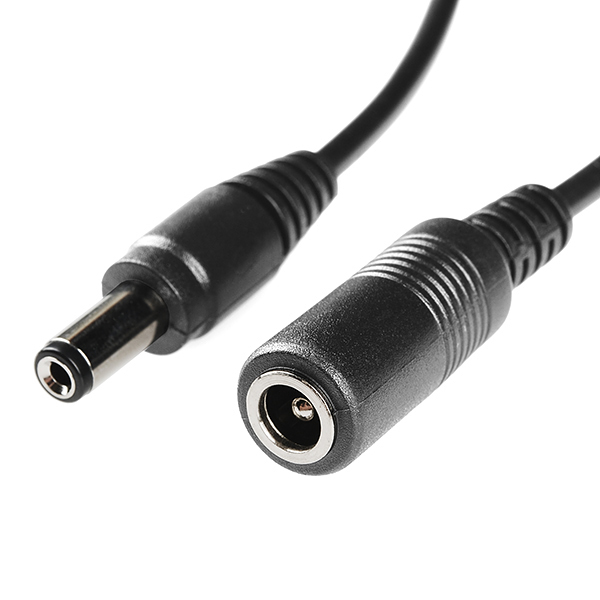
\includegraphics[height=0.9in]{imgs/connector_barreljack.jpeg}
\subcaption{Barrel Jack}
\end{subfigure}
\caption{Quick disconnect connectors.}
\end{figure}

\begin{asparaenum}[a)]
  \item \textit{Header pin connectors} or \textit{servo connectors} are simple, cheap connectors. They are commonly found on hobby servos. They don't have any locking features, though, so loosening is a major concern.
  \item \textit{Tabbed connectors} are simple crimp-on connectors. There are male and female sides which connect together. Shrouded versions which prevent shorting also exist.
  \item \textit{Locking connectors} come in many brands and styles. They feature a locking tab for quick and easy assembly, with positive latching.
  \item \textit{Waterproof connectors} are like locking connectors, but feature gaskets to keep moisture out from the wires and pins.
  \item \textit{Anderson connectors} are a type of \textit{hermaphroditic connector}- meaning there is no male or female side, so only one version of the connector is needed. These connectors have a snap feature, so they can be easily connected and disconnected, but there is nothing to positively keep them from coming apart. They can be zip tied together, however.
  \item \textit{D-sub connectors} are commonly associated with antiquiated serial ports, but their application is not limited to this. They can be screwed positively together, making them quite common on industrial equipment to this day.
  \item \textit{Screw on connectors} are circular, multiconductor connectors that can screw together to prevent them from coming apart.
  \item \textit{Barrel jacks} are very simple, easy to connect and disconnect, two-conductor connectors. While they are cheap, there is no good way to secure them, making them ill-suited to mobile use.
\end{asparaenum} 

\section{Communication Protocols}

\subsection{Dumb signals} % High/low, PWM

\begin{asparaenum}[a)]
\item Simple high and low signals can convey whether something is active or inactive at a particular point in time.
\item Analog signals can convey a particular variable value rather than a high or low. However, they require complex circuits to encode and decode from digital devices
\item \textit{Pulse-width modulation (PWM)} allows for the unidirectional trasmittal of variables over one signal wire without the need for analog circuitry. A square wave of fixed \textit{frequency} is generated and the variable to be sent is encoded in the \textit{pulse width} or \textit{duty cycle}. Typical "servo style" PWM uses a frequency of 50 Hz (or a period of 20 ms), with a pulse width of 1 ms corresponding to the minimum value (full reverse, or 0 degrees), and 2 ms corresponding to the maximum value (full forwards, or 180 degrees). This is a reasonably safe signal to send safety critical functions on as any interruptions to the signal would result in clearly invalid data.
\end{asparaenum}

\subsection{Serial links} % RS232, USB, UART, TTL

Serial encoding of data takes a binary signal and serializes it. For example, the ASCII character `A' is represented in binary as 01000001. So, one device would send a low signal, then a high signal, followed by five low signals, and a final high signal in order to transmit an `A'. Serial transfer is essential unidirectional, so if two devices want to communicate back and forth, two signal wires (along with a ground) will be needed.

\begin{figure}[H]
  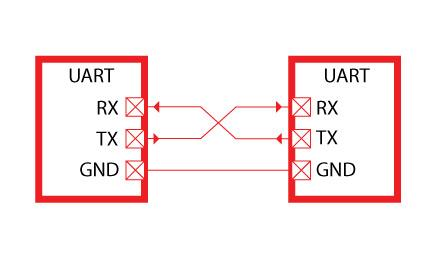
\includegraphics{imgs/setup_uart.jpeg}
  \caption{Basic serial wiring for bidirectional communication.}
\end{figure}

It isn't quite this simple, though- and so first-time users of raw serial protocols can often get quite frustrated as to why their devices won't connect.

To begin with, data is not always going to be transmitted over the line. The line will be a constant value before the data to be transmitted is sent. The sending device must first send a \textit{start bit} to denote the beginning of a transmission. Additionally, a \textit{stop bit} may be sent to denote the end of the transmission.

The devices need to agree in how many bits will be sent in a frame. Usually this is 8 bits, but 7 is possible (as is theoretically any number).

The two communicating devices must also be on the same frequency. There are many standard frequencies, or \textit{baud rates}. 

All signals also bear the possibility that they are degraded or contain errors. Use of \textit{parity} may be used to check for corruption. Parity is established by counting the number of high bits in the transmission, and then adding another bit at the end of the transmission to bring the count of high bits to an even number of bits (known as \textit{even parity}). The receiving device can then check if it recieved a transmission with an even number of bits- if the number was odd, the data got corrupted. If it is even, there's still a chance it was corrupted (maybe two bits flipped, cancelling the effect out), but a reduced one. \textit{Odd parity} also exists, working on the same principle, but with the aim of sending an odd number of bits.

The voltage levels are also important. The RS232 standard is for a logic low to be +9 to +25 volts, and a logic high to be -9 to -25 volts (note that this is inverse from what you might think!). This can fry a UART chip, which uses transistor-level voltages (usually either 5 or 3.3 volts), with 0 volts being a low and the transistor-level voltage being high.

\textit{USB} is another standard that builds on the idea of a serial link- although its wiring and protocol is much more complex.

\subsection{Bus signals} % I2C, SPI, CAN

Let's say, though, you want to build a network of devices. One topology to do this with would be a \textit{data bus}. This works by stringing all the devices together on a common set of wires.

\begin{figure}[H]
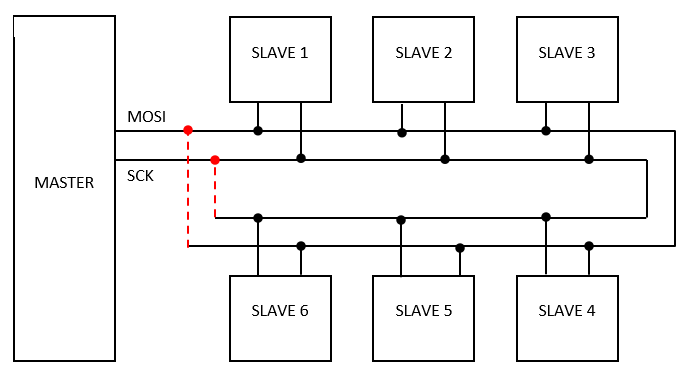
\includegraphics[width=0.8\textwidth]{imgs/bus_spi.png}
\caption{SPI bus}
\end{figure}

To send a communication, a device would put out a packet containing an intent to send information and its intended recipient, before sending the data. During this time, no other device can send data. The wiring of such a system is very simple and allows for the transmittal of sophisticated data, but does have bandwidth limitations and devices cannot simply hog the bus for extended periods of time.

There are many technical details and reasons to pick a particular bus technology or standard. The most prevalent are \textit{I2C}, \textit{SPI}, and \textit{CAN (Controller-Area-Network)}

CAN can be used in various topologies, or even a mix of them.

\begin{asparaenum}[A]
  \item In \textit{ring} or \textit{loop} topology, the devices are wired fully together, forming a loop. A \textit{terminating resistor} of 120 $\Omega$ is needed to connect the two lines of the bus together.
  \item In \textit{bus} topology, the devices are wired one to another, forming a line. Terminating resistors should be connected at either end of the bus.
  \item In \textit{star} topology, one master device or node is connected to all other devices, which would have their own terminating resistors. This may require more wire, but can be advantageous in that if one device becomes disconnected, the bus is not rendered inoperable to the other devices.
\end{asparaenum}